%Copyright (c) 2004 2005 2006 Atos Origin
%Permission is granted to copy, distribute and/or modify this
%document
%under the terms of the GNU Free Documentation License,
%      Version 1.2
%      or any later version published by the Free Software
%      Foundation;
%      with no Invariant Sections, no Front-Cover
%      Texts, and no Back-Cover
%      Texts.  A copy of the license is
%      included in the section entitled "GNU
%      Free Documentation License".
%
% $Id: overview.tex,v 1.3 2006/03/29 14:06:07 goneri Exp $
\documentclass[a4paper]{article}


\usepackage[latin1]{inputenc} % LaTeX, comprends les accents !
\usepackage[T1]{fontenc}      % Police contenant les caract�res fran�ais
\usepackage{geometry}         % D�finir les marges
\usepackage[francais]{babel}  % Placez ici une liste de langues, la
\usepackage{hyperref}
\usepackage{graphicx}  % picture incusion 
\usepackage{url}
\usepackage{color}
\usepackage{fancyhdr}
\pagestyle{fancy}
\usepackage{float}
%\floatstyle{ruled}
%\newfloat{figure}{thp}{lop}
\newfloat{figure}{!htb}{lop}
\floatname{figure}

\date{Janvier 2006}
\title{Pr\'{e}sentation de QSOS}
% title param :  title, author, date
\begin{document}

\renewcommand{\footrulewidth}{0.5pt}

\renewcommand{\arraystretch}{1.75} 
\setlength{\tabcolsep}{10pt}

% MACRO
% TabluarStrong : for tabular colonne title
\newcommand{\TS}[1]{\textbf{#1}}

\section{Pr\'{e}sentation de QSOS}
QSOS est une m\'{e}thode con\c{c}ue pour qualifier, s\'{e}lectionner et
comparer les logiciels open source. Elle est mise \`{a} disposition de la
communaut\'{e} sous licence libre GNU Free Documentation License.

\begin{figure}
\center
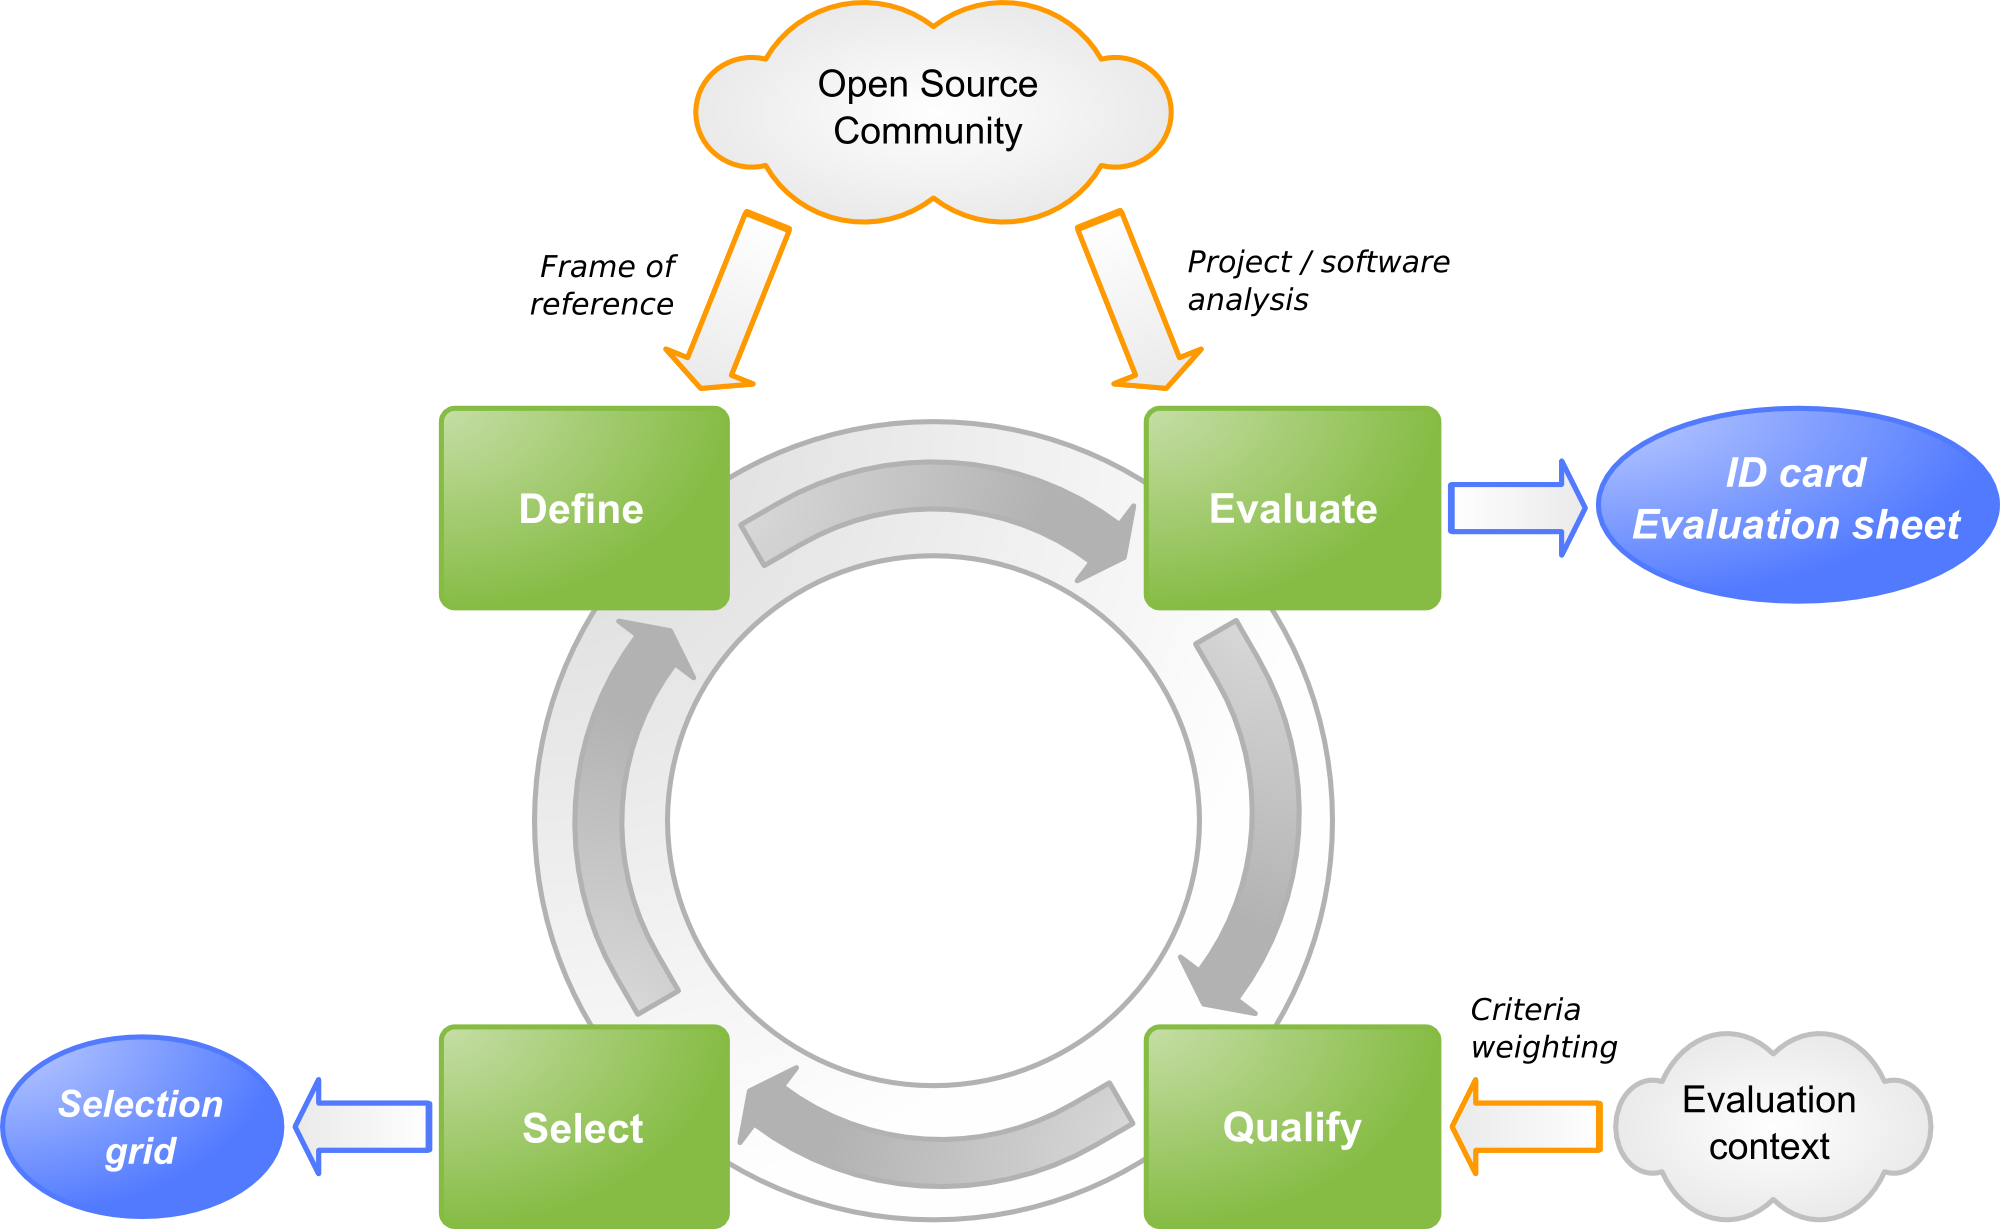
\includegraphics[width=13cm]{images/fr/processus_4_etapes}
\caption{D\'{e}finir}
\end{figure}


QSOS consiste en un processus it\'{e}ratif en quatre \'{e}tapes :

\begin{itemize}
\item D\'{e}finir les donn\'{e}es de r\'{e}f\'{e}rentiel (types de licences, types
de communaut\'{e}s, grilles de couverture fonctionnelle par domaine, ...)
\item �valuer les logiciels selon trois axes principaux : couverture fonctionnelle,
risques du point de vue de l'entreprise utilisatrice, risques du point de vue
du fournisseur de services (expertise, formation, support). Chaque axe est
constitu\'{e} d'un certains nombre de crit\`{e}res. Par exemple, l'axe des
risques entreprise comprend : la p\'{e}rennit\'{e} intrins\`{e}que,
l'int\'{e}gration, l'adaptabilit\'{e} technique, le niveau d'industrialisation
et la strat\'{e}gie du projet. Ces crit\`{e}res \'{e}tant eux-m\^{e}me
compos\'{e}s de sous-crit\`{e}res.
\item Qualifier le contexte sp\'{e}cifique d'une entreprise (ou d'un utilisateur) en
effectuant une pond\'{e}ration des crit\`{e}res pr\'{e}c\'{e}dents.
\item S\'{e}lectionner et comparer les logiciels r\'{e}pondant aux besoins.
\end{itemize}


Ce processus g\'{e}n\`{e}re des fiches d'identit\'{e}s de logiciel ainsi que
des grilles de comparaison et de choix. La d\'{e}marche par \'{e}tape, les
multiples crit\`{e}res d'analyse, et la m\'{e}trologie d\'{e}finis par QSOS en
font une m\'{e}thode qui permet une \'{e}valuation objective et argument\'{e}e
des logiciels libres pr\'{e}cieuse notamment dans des phases amont
d'\'{e}tude d'opportunit\'{e} de migration vers les logiciels libres ainsi que
pour choisir une solution open source optimale dans un contexte donn\'{e}.



\end{document}
% vi:syntax=tex
